\chapter{Exemplu de utilizare: Smart Home}
\label{chapter:studiuCaz}

Pentru a demonstra fiabilitatea platformei, acest capitol propune o soluţie pentru problema automatizării unei case. O asemenea soluţie, ieftină şi uşor de implementat încă lipseşte de pe piaţă, sistemele profesionale fiind foarte scumpe, iar cele open-source greu de instalat şi configurat.

Urmărim deci rezolvarea automatizării unei case cu un dormitor si o sufragerie, în care următoarele dispozitive au fost instalate:
\begin{itemize}
	\item Reţea de senzori inteligenţi, distribuiţi în toate camerele, capabili să ofere informaţii legate numărul de oameni din casă.
	\item Sistem de iluminare inteligentă, controlabil de la distantă.
	\item Un dispozitiv automat de închidere a uşii de la intrare.
\end{itemize}
Automatizarea constă în:
\begin{itemize}
	\item Atunci când nu mai exista oameni în casă, uşa trebuie încuiată;
	\item După un minut de când nu se mai află nimeni într-o camera lumina din acea cameră trebuie stinsă.
	\item Uşa se încuie automat la ora 00:00, dacă toţi oamenii se află în dormitor.
\end{itemize}

Au fost create următoarele blocuri de intrare, pentru fiecare dispozitiv:
\begin{itemize}
	\item \textbf{Prezenţă Sufragerie}: indică dacă exista oameni in sufragerie. Are un singur canal, pe care trimite date de tip întreg despre numărul de oameni din cameră.
	\item \textbf{Prezenţă Dormitor}: senzorul din dormitor, analog cu Prezenţă Sufragerie.
\end{itemize}
\begin{figure}[H]
	\centering
	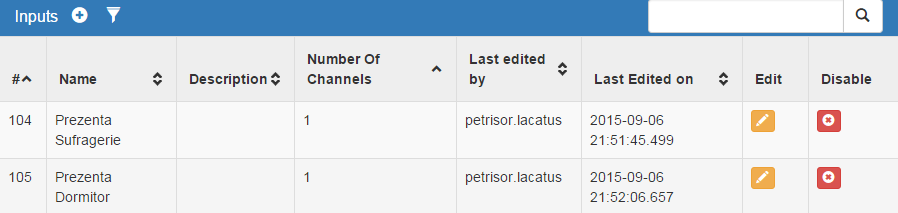
\includegraphics[width=1.1\textwidth, center]{utilizare/inputs}
	\captionsetup{justification=centering}
	\caption{Intrările in aplicaţie}
	\label{fig:inputs}
\end{figure}

Următoarele diagrame au fost implementate:
\begin{itemize}
	\item \textbf{Închidere uşă noaptea}: Comandă închiderea uşii după ora 00:00 dacă toţi oamenii sunt în dormitor;
	\item \textbf{Securizare casa}:  Comandă închiderea uşii când senzorii de prezenţă indică faptul că nu mai sunt oameni \ref{fig:securizareCasa};
	\item \textbf{Oprire lumina dormitor}:  Comandă oprirea luminii când nu mai e nimeni în dormitor;
	\item \textbf{Oprire lumina sufragerie}: Analog, pentru sufragerie;
\end{itemize}

\begin{figure}[H]
	\centering
	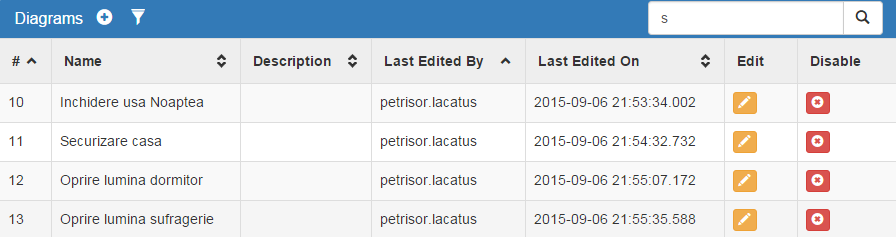
\includegraphics[width=1.1\textwidth, center]{utilizare/diagrams}
	\captionsetup{justification=centering}
	\caption{Diagramele implementate}
	\label{fig:diagrams}
\end{figure}

\begin{figure}[H]
	\centering
	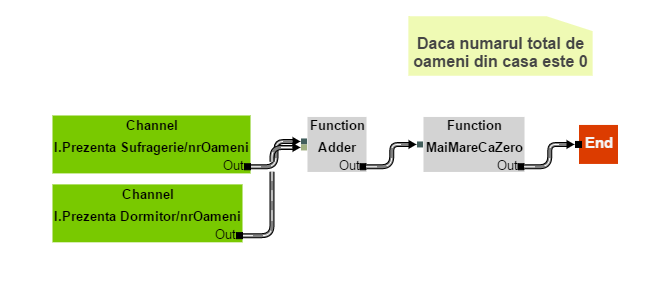
\includegraphics[width=1.1\textwidth, center]{utilizare/securizareCasa}
	\captionsetup{justification=centering}
	\caption{Diagrama pentru securizarea casei}
	\label{fig:securizareCasa}
\end{figure}